
\documentclass[linenumbers,draft]{agujournal}
\journalname{Tectonics}
\usepackage{soul}
\usepackage{breakcites}
\begin{document}

\title{Late Holocene structural style and seismicity of highly transpressional faults in southern Haiti}

\authors{Jiannan Wang, Paul Mann, Robert R. Stewart}
\affiliation{}{Department of Earth and Atmospheric Sciences, University of Houston, Houston, Texas, USA.}

\correspondingauthor{Jiannan Wang}{jwang61@uh.edu}

\begin{keypoints}
\item First high-resolution sonar surveys of two actively deformed lakes in Haiti.
\item High degree of regional, tectonic transpression is partitioned by $en~echelon$ thrust faults and associated folds adjacent to a major strike-slip, plate boundary fault.
\item Estimates of relative ages of deformation of major strike-slip faulting and $en~echelon$ thrusts from deformed and undeformed lake sediments.
\item 3D deformation model integrates patterns of 2010 coseismic uplift, aftershock distribution, and mapped geologic structures.
\end{keypoints}

\begin{abstract}
The devastating 2010 Haiti earthquake ($M_w$ 7.0) was caused by rupture of the L\'eog\^ane, blind, thrust fault located 5 km north of the main, Caribbean-Gon\^ave plate boundary, a 1200 km-long, left-lateral, Enriquillo-Plantain Garden fault zone (EPGFZ). Unexpectedly, the EPGFZ, which remained largely quiescent or slightly reactivated during the 2010 earthquake, although, formed a boundary between a coseismically uplifted lowland north of the EPGFZ and a subsided area in the highlands south of the fault. Here, we use high-resolution sonar data from two, Haitian lakes that straddle the EPGFZ and its northern flank to demonstrate the presence of a 10 -- 15 km-wide, 120 km-long, late Holocene fold-thrust belt which deforms clastic, lowland basins along the northern edge of the EPGFZ. In the eastern part of the study area, sonar results from Lake Azuey show that the linear trace of the EPGFZ cutting the Holocene lake bed is more deeply buried and less active than the adjacent, newly discovered, northwest-striking, northeast-dipping Jimani thrust fault that is part of the adjacent transpressonal belt of $en~echelon$ thrust-and-fold. This structural relationship between a less active EPGFZ and more recently active, transpression-related Jimani thrust is remarkably similar to the 2010 epicentral area 70 km to the west between the less active EPGFZ and seismogenic L\'eog\^ane thrust during the 2010 Haiti earthquake. In this complex transpressional zone, we propose that coseismic deformation alternates at recurrence intervals of centuries between oblique, transpression-related structures (L\'eog\^ane, Jimani, and Trois Baies blind thrusts) and the main strike-slip, plate boundary fault zone (EPGFZ).
\end{abstract}

\section{Introduction and tectonic setting of the 2010 Haiti earthquake}
\label{sec:intro}
On January 12, 2010, a $M_w$ 7.0 earthquake struck the densely populated, greater Port-au-Prince region of south-central Haiti and caused widespread destruction with over 230,000 fatalities and an estimated 10 billion dollars damage \citep{prentice2010seismic,bilham2010lessons,paultre2013damage,kocel2016near} (Figure \ref{figure1}). Multidisciplinary, geological and geophysical studies of the 2010 epicentral area of south-central Haiti including: 1) coseismic, coral reef uplift observation along a 50 km-long area of coastline in the epicentral region combined with fault modeling \citep{hayes2010complex}; 2) coseismic, vertical ground motion from radar interferometry \citep{hashimoto2011fan}; 3) high-resolution, surface-fault-trace mapping using Light Detection And Ranging (LIDAR) and targeted field studies \citep{cowgill2012interactive}; 4) Global Positioning System (GPS) and 2010 aftershock-based studies and modeling of pre-, syn-, and post-2010 earthquake crustal motions \citep{calais2010transpressional,nettles2010earthquake,symithe2013coseismic,douilly2013crustal,douilly2015three}; 5) ground-based studies of Holocene scarps including coseismic ground fractures and late Quaternary scarps of the EPGFZ that remained unaffected by 2010 fault breaks \citep{prentice2010seismic,koehler2011field,rathje2014geotechnical,saint2015seismotectonics}; 6) ground-based, near-surface, geophysical surveys of buried faults activated during the 2010 earthquake \citep{kocel2016near}; 7) near-coast surveys of submarine extensions of faults active in 2010 \citep{hornbach2010high,mercier20112010}; and 8) deepwater, marine surveys and coring to determine the recurrence interval of major earthquakes based on anomalous sedimentary deposits related to shaking and increased erosion \citep{mchugh2011offshore}.

The consensus from these previous, on- and offshore, multidisciplinary studies is that the 2010 earthquake ruptured two, previously unrecognized west- to northwest-striking thrust faults located 2 to 5 km north of the 1200 km-long, left-lateral, Enriquillo-Plantain Garden fault zone (EPGFZ) that forms a major, plate boundary between the Caribbean plate to the south and the Gon\^ave microplate to the north \citep{mann1995actively,calais2010transpressional,benford2012gps,corbeau2016transpressive} (Figure \ref{figure1}A, B). These two thrust are separated by 6 km and include: 1) the subaerial, 8 km-long, blind, L\'eog\^ane thrust fault located 5 km north of the EPGFZ and trending at an angle of $8^{\circ}$ to the EPGFZ \citep{calais2010transpressional,douilly2013crustal,douilly2015three}; and 2) the submarine, 20 km-long Trois Baies thrust fault located 2 km north of the EPGFZ and trending at an angle of $20^{\circ}$ \citep{mercier20112010,symithe2013coseismic} (Figure \ref{figure1}B, C).

Despite the proximity of the L\'eog\^ane and Trois Baies thrust to the neighboring EPGFZ, the EPGFZ remained largely quiescently and outside the zone of maximum, coseismic uplift and ground shaking and aftershocks related to the 2010 earthquake \citep{nettles2010earthquake}. The centroid moment tensor (CMT) mechanism of the main 2010 shock shows a primarily strike-slip motion, with a small component of reverse motion, on a steeply north-dipping nodal plane \citep{nettles2010earthquake,douilly2013crustal}. Finite element modeling \citep{douilly2015three} suggests that L\'eog\^ane fault buried beneath at least 1 km of overlying undeformed clastic sediment in the area north of the EPGFZ absorbed most of the energy of the northwest-southeast compression along obliquely-striking, high-angle ($21^{\circ}$-$70^{\circ}$ dipping) reverse fault planes, leaving significantly increasing but insufficient stress to trigger a 2010, coseismic slip on the adjacent EPGFZ 5 km to the south (Figure \ref{figure1}B). Previous GPS surveys by \citet{calais2010transpressional,calais2016plate} show along this area of the EPGFZ display vectors at almost right angles to these obliquely-striking thrusts and consistent with their preferred reactivation (Figure \ref{figure1}A, B).

Aftershock studies following the 2010 earthquake by \citet{douilly2013crustal,douilly2015three} showed that the EPGFZ moved slightly at depth and acted as a 6 km-long, east-west and sub-vertical, connecting fault segment that transmitted seismogenic motion between the obliquely-trending, south-dipping, L\'eog\^ane fault in the east and the more obliquely-trending, northeast-dipping Trois Baies fault in the west (Figure \ref{figure1}B). However, post-earthquake geologic reconnaissance revealed no surface ground breaks along the proposed onland areas of EPGFZ motion in the epicentral region of the earthquake \citep{prentice2010seismic,koehler2011field,rathje2014geotechnical}. A more recent study by \citet{saint2015seismotectonics} proposed previously, unrecognized, 2010 coseismic groundbreaks along the obliquely-trending Lamentin thrust 11 km east of the epicentral area near the city of Port-au-Prince (Figure \ref{figure2}A).

Oblique, $en~echelon$ thrusts spacing at distances of 1-8 km along the main strike-slip fault, obliquely intersect the main strike-slip fault at angles of $30^{\circ}$-$45^{\circ}$ and strike northwestward away from the EPGFZ with individual oblique, fault lengths extending into the deeper basins at distances of 4-29 km (Figure~\ref{figure2}A, Figure~\ref{figure3}).  As a result of this distinctive and regular intersecting fault geometry between these oblique thrusts and the linear and continuous EPGFZ, earthquake rupture initiating on an oblique thrust, as seen for the L\'eog\^ane fault in 2010, is likely confined to that vicinity and may not connect with other oblique thrusts or even the EPGFZ itself \citep{douilly2013crustal,douilly2015three}.

Coseismic deformation along a large transpressional strike-slip fault, such as the EPGFZ and Septentrional \citep{calais2002strain} in Hispaniola or the San Andreas fault zone in California \citep{segall1990surface}, either is accommodated by slip and major earthquakes on the main, strike-slip plate boundary fault, or is accommodated by the oblique, $en~echelon$ thrusts adjacent to the main fault, or is accommodated by both sets of faults (cf. compilation of types of destructive earthquakes in transpressional settings by \citet{hayes2010complex}). Motions on distributed, $en~echelon$ thrusts do not necessarily spare or reduce coseismic rupture on the main strike-slip fault because the $en~echelon$ and main strike-slip fault remain separate fault planes, and the main strike-slip fault could continue to accumulate strain. In an extreme case, plate motions become increasingly transpressional as seen in the case of the EPGFZ as manifested in the obliquity of GPS vectors relative to the strike of the EPGFZ (Figure~\ref{figure1}A, B) or in a restraining bend setting or during the plate reorganizations. In this settings, the $en~echelon$, oblique thrusts might assume more and more plate-edge strain to the point that the plate boundary behaves more like a thrust belt and less like a strike-slip boundary.

These oblique and $en~echelon$ thrust faults in transpressional settings, including large restraining bends like Hispaniola, potentially nucleate ``uncharacteristic earthquakes'' of varying recurrence intervals and sizes that are distinct from the recurrence intervals and sizes of the adjacent but independent strike-slip fault \citep{Fielding2013}. Restraining bend areas like Hispaniola can lead to the generation and increased activities on more favorably and obliquely oriented folds and thrusts whose coseismic rupture might alternate with much longer ruptures along the adjacent strike-slip fault. The number of these $en~echelon$, thrust faults can be large at observed spacing of 5-10 km along strike-slip faults that may be hundreds of kilometers in total length. For this reason, the identification of oblique thrusts in $en~echelon$ sets, especially when buried or ``blind'', can be challenging, along with assessing their role in seismogenesis within a broad plate boundary and their recurrence intervals pose a major challenge for seismic hazard assessment in areas of regional transpression like Hispaniola \citep{frankel2011seismic}.

\section{Objectives and methods}
The objective of this paper is to better integrate the geologic structure of the 120 km-long study area, that parallels the trace of the EPGFZ and includs the 2010 epicentral area, using a wealth of geologic, geophysics, GPS, radar interferometry, aftershock, and modeling studies, most of which has been collected since the 2010 earthquake. Our main objective is to use these information to structurally characterize the 10-15 km-wide, belt of late Holocene, transpressional deformation that forms a laterally-persistent, deformed belt along the inland, Cul-de-Sac intermontane basin in the east and the low-relief coastal plain along Port-au-Prince bay and the Canal du Sud to the west \ref{figure1}B. In particular, we focus on the identifying a family of $en~echelon$ thrusts, whose curvilinear strikes area are very similar to the L\'eog\^ane thrust now known to be responsible for most of the energy release and coseismic uplift during the 2010 Haiti earthquake \citep{calais2010transpressional,douilly2013crustal,douilly2015three} (Figure \ref{figure1}B, Figure \ref{figure2}A).

This elongate, belt of transpressional deformation associated with $en~echelon$ thrusts occupies a topographically-low, densely populated Cul-de-Sac basin underlain by poorly consolidated clastic sedimentary rocks ranging in age from Miocene to recent \citep{massoni1955haiti,mann1995actively,terrier2014revision,saint2015seismotectonics}. In easternmost Haiti, this belt is overlain by the the shallow (33 m), 138 km\textsuperscript{2}, brackish Lake Azuey near the border separating Haiti from the Dominican Republic \citep{wright2015factors,piasecki2016bathymetric}. Lake Enriquillo to the east is a larger, shallow (52 m), 346 km\textsuperscript{2}, hypersaline, sub-sealevel lake located entirely in the Dominican Republic and separated from Lake Azuey by the eastward continuation of the same transpressional belt parallel and north of the EPGFZ in the Cul-de-Sac valley \citep{mann1995actively} (Figure \ref{figure1}B). 

In the western part of our study area, the more transtensional segment of the EPGFZ is overlain by the the 42.8 m-deep, 14 km\textsuperscript{2}, freshwater Lake Mirago\^ane (Figure \ref{figure1}B). All three of these shallow, inland, lakes experience variations up to 13 meters in their surface elevations due to annual to decadal changes in climate and rainfall amounts including extreme rainfall associated with hurricanes \citep{wright2015factors,piasecki2016bathymetric,moknatian2017development,rico2017hydrodynamic}.  
  
In order to understand the geologic and structural styles of transpression within this belt, including the age relations between deformation in the north-flanking belt and the EPGFZ itself, we collected a total of 94 km of high-resolution (2-10 kHz) sonar profiles in 2014 from the 138 km\textsuperscript{2}, brackish Lake Azuey (Figure~\ref{figure2}A, B) and 37 km of profiles from the 14 km\textsuperscript{2}, fresh-water Lake Mirago\^ane (Figure~\ref{figure1}B). The EPGFZ strikes through both of the lakes, so 80\% of our grid on Lake Azuey and 90\% of our grid on Lake Mirago\^ane was dedicated to the across fault-strike, north-south profiles (Figure~\ref{figure1}B). 

The average speed of the boat towing the sonar was 3 knots, and we used a sonar pulse rate of 4 per second. Our 2-10 kHz sonar frequency range gives sub-bottom layer resolution of about 10 cm. These surveys were the first sonar surveys in Haitian lakes. Both lakes straddle the active trace of Haiti's EPGFZ and its adjacent, transpressional fold-thrust belt, therefore provide new constraints on the location, structural style, and timing of deformation within both structural provinces. We incorporate these lake data with previous geologic mapping, geophysical observations related to the 2010 earthquake, and regional information on plate motions in this region (Figure~\ref{figure1}B). 

\section{Tectonic setting of transpressional deformation in south-central Haiti including unresolved tectonic and structural questions}
\label{sec:tectonic}
\subsection{Previous strike-slip deformational model vs. Haiti thrust belt deformational model}
There are two regional structural models to explain the present-day structure of the broad, 250 km-wide zone of transpression spanning the entire width of the island of Hispaniola.

\subsubsection{Strike-slip, regional structural model}
The first is the strike-slip-dominated model, driven by oblique motion and transpression between the thick and buoyant Bahama platform on the North America plate, the Caribbean plate, and the Gon\^ave plate \citep{mann1995actively,dolan1998active,mann2002oblique,calais2002strain,calais2016plate} (Figure \ref{figure1}A, B). Structures and tectonic geomorphology formed in this 250 km-wide, transpresssional zone include: 1) strain partitioning along the EPGFZ and the subparallel Septentrional strike-slip fault zone along the north side of the island as known from GPS studies \citep{calais2002strain,calais2010transpressional,hayes2010complex,symithe2013coseismic,douilly2013crustal,douilly2015three}; 2) as a result of transpression, the central Hispaniola has the highest topography, up to 3 km, in all of the northern Caribbean region; 3) left-lateral strike-slip rupture of the EPGFZ in the 18th century inferred from historical earthquakes \citep{bakun2012significant} with average left-lateral offset amounts of 1.3 -- 3.3 m as expressed along offset streams of the EPGFZ \citep{prentice2010seismic} and by left-lateral, channel offsets of 7 -- 8 m along stream channels by the Septentrional fault zone \citep{prentice1993paleoseismicity}; 4) folding and thrusting of 10 -- 15 km-wide belt of Miocene to Quaternary rock adjacent to the EPGFZ \citep{saint2015seismotectonics}; and 5) a strong, southwestward, backthrusting of the Gon\^ave microplate, in southern Hispaniola in Haiti and Dominican Republic to the southwest onto the Caribbean plate \citep{mann2002oblique,grindlay2005high,kroehler2011late} (Figure \ref{figure1}B, C). Southwestward backthusting of Hispaniola is manifested by the accretionary wedges present along the Muerto trench south of the Dominican Republic \citep{bien1986contribution,bruna2009morphotectonics} (Figure \ref{figure1}B) and along the southern margin of Haiti (South Haiti accretionary prism \citep{bien1986contribution} (Figure \ref{figure1}C), along with the associated, localized, negative gravity anomaly associated with plate flexure under a thrust load \citep{mann2002oblique,bruna2009morphotectonics} (Figure \ref{figure1}A)).

\subsubsection{Criticisms of the strike-slip, regional structural model}
Two criticisms have been proposed for the strike-slip model. First, \citet{corbeau2016transpressive} has questioned whether the predictions of the GPS-based block models, which predict significant shortening, are accurate that little transpression-related shortening can be observed from regional seismic profiles in the offshore area of the Gulf of Gon\^ave north of the southern peninsula of Haiti, or in the area of the Jamaica Passage east of Haiti. Second, \citet{symithe2016present} have proposed that there is no geologic evidence for a continuation of the EPGFZ east of latitude $72.27^{\circ}$W in the eastern Cul-de-Sac Valley, Lake Azuey and Lake Enriquillo in the Dominican Republic (Figure~\ref{figure1}B). Instead, \citet{symithe2016present} propose that large rates of north-south shortening predicted from GPS block models is taken up entirely by low-angle thrust structures in the eastern Cul-de-Sac and Enriquillo Valleys that were modeled using GPS data as part of their study.

\subsubsection{Trans-Haitian fold-and-thrust belt regional structural model}
The Trans-Haitian fold-and-thrust belt model originated with a study by \citet{pubellier2000plate}, who proposed a low-angle southwestward-verging fold-and-thrust belt along the southwestern edge of the central Hispaniola block. The thrust front of this feature was thought to be actively propagating from the main Trans-Haitian fold-and-thrust belt, located in the Cha\^ine des Matheux, southwestward into the area of the L\'eog\^ane plain and the Cul-de-Sac basin, further more, emerging into, as what we are proposing in this paper, the transpressional belt along the northern flank of the EPGFZ (Figure \ref{figure2}A, B). \citet{pubellier2000plate} proposed that the EPGFZ originally formed as a left-lateral strike-slip fault, but became inactive in the late Miocene when deformation in southern Hispaniola became compressional and the Trans-Haitian fold-and-thrust belt had propagated into the southern area of the Cul-de-Sac basin and L\'eog\^ane plain, where it emerged or ``daylighted'' to form the $en~echelon$, convergent structures (compiled on the map in Figure \ref{figure2}). \citet{pubellier2000plate} also proposed that the EPGFZ was reactivated as a normal fault in the Quaternary as a result of crustal loading of the southern, foreland area by the overthrusting Trans-Haitian fold-and-thrust belt. 

Following the 2010 earthquake and the recognition of the north-dipping blind L\'eog\^ane thrust fault, \citet{calais2010transpressional} proposed that this fault is the leading edge of the Trans-Haitian fold-and-thrust belt rather than being an $en~echelon$ thrust genetically linked to the EGPFZ, as we propose in this paper based on the geologic data compiled on Figure~\ref{figure2}A, B. In the interpretation proposed by \citet{calais2010transpressional}, the northward dip of the L\'eog\^ane thrust made it difficult to link its origin with the EPGFZ, whose dip had been established in this area as a vertical to high angle (> $60^{\circ}$), south-dipping fault plane with evidence of late Holocene, left-lateral offsets of drainages \citep{prentice2010seismic}. Moreover, \citet{symithe2016present} noted that Trans-Haitian fold-and-thrust belt regional model of \citet{pubellier2000plate} was more consistent with an increasing amount of GPS data supportive of a larger magnitude, north-south shortening in central Hispaniola than with the existence of an eastward extension of the left-lateral EPGFZ into the eastern part of Haiti and the Dominican Republic (Figure~\ref{figure1}B and Figure \ref{figure2}A).

\subsubsection{Criticisms of the Trans-Haitian fold-and-thrust belt, regional structural model}
First, \citet{mercier20112010} pointed out two problems with linking the origin of the L\'eog\^ane thrust to the southwestward-propagating edge of the Trans-Haitian fold-and-thrust belt: 1) the dip of the fault generating the main thrust, derived by the \citet{mercier20112010}, was more steeply dipping ($64^{\circ}$) than expected for a blind thrust at the leading edge of a fold-thrust belt; and 2) the orientation of the N$84^{\circ}$E fault plane of the main shock is significantly oblique to the N$120^{\circ}$E-oriented leading edge of the Trans-Haitian fold-and-thrust belt as proposed by \citet{pubellier2000plate}. In this paper we discuss other inconsistencies with the zone of deformation north of the EPGFZ being the result of southwestward propagation of the Trans-Haitian fold-and-thrust belt.

\section{New observations of the Late Holocene structural style along EPGFZ in southern Haiti}
\subsection{Significance of $en~echelon$ thrusting and folding north and south of the EPGFZ}
The presence of a strike-slip fault at any scale is indicated by the presence of $en~echelon$ arrays of thrust faults, normal faults, folds, fractures, dikes, and other linear features in narrow, elongate zones \citep{sylvester1988strike}. On Figure \ref{figure2}A, we have compiled geologic information on $en~echelon$ folds and faults in a 10 -- 15 km-wide zone of deformation along both the northern and southern flanks of the EPGFZ. Folds form as fault propagation folds along oblique thrust faults, vary from 1 to 8 km in lateral spacing; and deform Miocene and younger fine to coarse-grained, basinal, and coastal plain rocks in the belt that is 10 -- 15 km wide and extends parallel to the EPGFZ for 120 km (Figure~\ref{figure1}B and Figure~\ref{figure2}A). Folds in Neogene clastic lithologies of the Cul-de-Sac basin contrast with more continuous and longer wavelength, $en~echelon$ fold axes present in more massively-bedded Cretaceous to Eocene rigid, basaltic, and carbonate lithologies exposed in the 2 km-high range south of the EPGFZ, the Massif de Selle (Figure~\ref{figure2}B). The trend of fold axes is similar to the north and south of the EPGFZ (Figure \ref{figure2}B). 

The $en~echelon$ distribution of complex Holocene folding and thrusting in the 10 -- 15 km wide zone of deformation north of the EPGFZ is also reflected in the complex pattern of 2010 coseismic and vertical deformation recorded by the interferogram from the 2010 epicentral area on the L\'eog\^ane plain west of the Cul-de-Sac basin \citep{hayes2010complex,hashimoto2011fan,bilham2013remote} (Figure \ref{figure2}A). \citet{douilly2013crustal,douilly2015three} and \citet{kocel2016near} use aftershocks and shallow geophysics to show that the 2010 L\'eog\^ane thrust fault and sub-parallel faults are overlain by at least one kilometer of undeformed and sub-horizontal strata.

\subsection{Significance of curvilinear fold and thrust patterns in the transpressional belt north of the EPGFZ}
The shaded relief DEM (digital elevation model) shown in Figure \ref{figure2}B reveals the curvilinear, $en~echelon$ fold morphologies that are defined by low, bedrock hills of Neogene sedimentary rocks exposed on the flat-lying Cul-de-Sac basin. These curvilinear fold axes can be related directly to a broad zone of left-lateral, simple shear produced along the sub-vertical and left-lateral EPGFZ based on several, basic observations seen on Figure~{figure2}B: 1) the most prominent folds are present along the southern edge of the Cul-de-Sac basin within 15 km of the EPGFZ; in contrast, the central and northern edges of the Cul-de-Sac basin exhibit no prominent folding even directly adjacent to the base of Eocene-Miocene carbonate rocks forming the range \citep{pubellier2000plate} (Figure \ref{figure2}A); 2) as typical broad zones of shearing on the thick, sedimentary rocks as shown schematically in the inset of Figure~\ref{figure2}B (modified from \citet{odonne1983analogue}), the fold axes along the southern margin of the Cul-de-Sac basin are asymptotic, or gently curve into east-west parallelism with the main trace of the EPGFZ along the southern edge of the Cul-de-Sac basin; 3) deeper, structural depressions form in the zone of convergent intersection between the east-west-striking EPGFZ and the northwest-striking, secondary thrusts as seen in the southern part of Lake Azuey, where the lake bends from an east-west trend adjacent to the EPGFZ to a more northwest trend in the central and northern part of the basin (Figure~{figure2}A, B); and 4) in our sonar mapping of Lake Azuey described below, we observed late Holocene lake sediments onlapping onto local highs of Eocene limestone of the bounding range along the northern edge of the lake with no evidence of late Holocene faulting or folding as observed with the EPGFZ along the southern edge of the lake (Figure \ref{figure2}A). 
%The broad, 250 km-wide zone of transpression spanning the entire width of the island of Hispaniola is driven by oblique motion between the North America, Caribbean, and Gon\^ave plates and includes: 1) the highest topography, up to 3 km in the northern Caribbean region; 2) strain partitioning along the EPGFZ and the subparallel Septentrional strike-slip fault zone along the north side of the island as known from GPS studies \citep{calais2010transpressional,hayes2010complex,prentice2010seismic,symithe2013coseismic,douilly2013crustal,douilly2015three}; 3) left-lateral strike-slip rupture of the EPGFZ in the 18th century inferred from historical earthquakes \citep{prentice2010seismic}; and 4) folding and thrusting of 10-15 km-wide belt of Miocene to Quaternary rock adjacent to the EPGFZ \citep{saint2015seismotectonics} (Figure~\ref{figure1}B, C).

On a more regional scale, these observations form Lake Azuey are consistent with the Canadian Superior 2D, multi-channel, seismic reflection profile (shown in Figure~\ref{figure1}C), that shows a lack of intensive deformation in the northern part of Port-au-Prince Bay, that is the offshore, largely un-faulted and folded seaward extension of the Cul-de-Sac basin \citep{mchugh2011offshore}. \citet{pubellier2000plate} proposes that the Trans-Haitian fold-and-thrust belt exposed in the Chaine des Matheux range north extends beneath the entire Cul-de-Sac and Port-au-Prince basins (Figure \ref{figure2}A, B). In summary, our observations at this scale do not support the previous model by \citet{pubellier2000plate} and \citet{calais2010transpressional} that folds and faults of the northern range are propagating southwestward beneath the zone of $en~echelon$ faults and folds (Figure \ref{figure2}A, B).

\subsection{Geologic structure of the area of $en~echelon$ thrusts in the epicentral area on the L\'eog\^ane fan-delta}
\subsubsection{Geologic structure of the L\'eog\^ane fan area}
A cross sectional profile of the 2010 epicentral area related to activation of two, conjugate thrust faults was modified from aftershock data from \citet{douilly2013crustal,douilly2015three} is shown in Figure \ref{figure3} (Line A--A'). Both faults are buried by about 1 km of late Quaternary sand and gravel of the L\'eog\^ane fan delta \citep{kocel2016near} and an additional 1 km of Paleocene limestone. Aftershocks indicate the main thrust event ruptured a depth range of from 4 to 17 km beneath the ground surface \citep{douilly2013crustal,douilly2015three}. The orientation of the L\'eog\^ane thrust based on gravity and uplift of coastal features is east-west and parallel to recent near-surface breaks of the EPGFZ mapped in the shallow, coastal zone adjacent to the L\'eog\^ane plain \citep{hornbach2010high}. Due to its proximity to the EPGFZ, an east-west strike of the L\'eog\^ane thrust is predicted as this is the area where $en~echelon$ folds and faults curve into an asymptotic orientation relative to the main EPGFZ, as shown on Figure \ref{figure2}B.

A radar interferogram compiled on the structure map of Figure \ref{figure2}A revealed that the 2010 earthquake elevated the smaller folds of the L\'eog\^ane fan-delta north of the EPGFZ, yet produced coseismic subsidence in the 1.4 km-high, less complexly deformed, mountain range south of the EPGFZ to the south \citep{hashimoto2011fan} (Figure \ref{figure2}A). This paradox can be simply explained by the northward dip of the seismogenic L\'eog\^ane fault that elevated the basinal area to the north (hanging wall of the L\'eog\^ane fault) and depressed the mountainous area to the south (footwall block of the L\'eog\^ane fault (line A--A' in Figure \ref{figure3}). 

\subsubsection{Geologic structure of the greater Port-au-Prince urban area compared to the L\'eog\^ane epicentral area} 
A similar pattern of deformation is observed in Port-au-Prince urban where the central and northern edge of the Cul-de-Sac basin is undeformed \citep{massoni1955haiti,cox2011shear,mchugh2011offshore,saint2015seismotectonics} (Line B-B' in Figure \ref{figure3}). The cross section taken from workers, who were mapping 60 years ago when the city was smaller and the geology was less obscured, shows two large thrusts, a range-bounding thrust along the southern edge of the city, and a north-dipping thrust, the Dumay thrust, that elevates a broad outcrop zone of north-dipping, Neogene sedimentary rocks on which the northern part of the city is built \citep{rathje2014geotechnical}. The $50^{\circ}$ northeast dip of the Dumay thrust is similar to the $70^{\circ}$ northeast dip of the L\'eog\^ane thrust to the west known from aftershocks \citep{douilly2013crustal,douilly2015three}, although the dip of the Dumay thrust reverses to a southwest dip as it approaches the EPGFZ (Figure~\ref{figure2}A, B). On the cross section B--B' in Figure~\ref{figure3}, we have schematically indicated areas that are elevated as a result of the northward dip of the Dumay thrust and the depression of the area to the south of the EPGFZ in the highlands south of the EPGFZ. If a future earthquake occurred along the north-dipping, $en~echelon$ thrust faults in the Port-au-Prince are (Line B--B' in Figure~\ref{figure3}) or Lake Azuey area (Line C--C' in Figure~\ref{figure3}) a similar uplift phenomenon would occur where the lowlands are uplifted and the adjacent mountains subside.

\subsubsection{Geologic structure of the Lake Azuey area} 
Structural cross-sections (Figure \ref{figure3}) from this and the previous works \citep{massoni1955haiti,bourgueil1988synthese,cox2011shear,douilly2015three} (Line A--A' and B--B' in Figure \ref{figure3}) along this 120 km-long zone of deformation adjacent to the EPGFZ show that the oblique thrust faults share a similar orientation with other north-dipping thrusts along the northern edge of the EPGFZ. All three of these oblique thrust faults shown on the cross sections deform rocks as young as Pliocene and Quaternary \citep{saint2015seismotectonics}. 

In our sonar survey of Lake Azuey, we observed that the most prominent folds present adjacent to the EPGFZ become less prominent in the central and northern parts of the lake (Figure \ref{figure2}B). These southern folds and thrusts imaged in Lake Azuey define the transpressive belt along the EPGFZ observed in onshore areas to the west. On the cross section C--C' in Figure~\ref{figure3}, we have schematically indicated areas that are elevated as a result of the northward dip of the Jimani thrust and the depression of the area to the south of the EPGFZ in the highlands south of the EPGFZ.

\subsection{Subsurface stratigraphy of Lake Azuey and Lake Enriquillo and paleoseismic estimates of the relative timing of recent earthquakes on the EPGFZ and secondary, $en~echelon$ thrust faults}
Our objective is to determine the relative age of the EPGFZ and its adjacent zone of fold-and-thrust deformation using the sonar profiles from Lakes Azuey and Enriquillo (Figure \ref{figure4}A). Both previous coring in Lake Enriquillo \citep{rios2013holocene}, which was tied to onshore stratigraphic studies \citep{taylor1985stratigraphy,rios2013holocene}, and in Lake Mirago\^ane \citep{higuera199910} have established the late Holocene to include the upper 5 and 7 meters of both lakes, respectively. 

Mapping in both lakes revealed the presence of the east-west strands of the EPGFZ that are collinear with online scarps both east and west of Lake Azuey (Figure \ref{figure2}, Figure \ref{figure4}, and Figure \ref{figure5}) and east and west of Lake Enriquillo \citep{mann1995actively,rios2013holocene}. These east-west fault strands abruptly truncate the trends of folds in the ranges south of the lake (Figure \ref{figure5}). 

In Lake Enriquillo, a sonar survey similar to ours was conducted in 2013 \citep{rios2013holocene}. The sonar events, which are interpreted as stratigraphic features, from Lake Azuey and Lake Enriquillo (Line B1 and Line L19 correlate convincingly (Figure \ref{figure4}B). Given the small distance separating the two lakes (about 4 km); the similarity of the stratigraphic profiles; and the same amount of sediment above the EPGFZ; it is reasonable to suggest that Lake Azuey and Lake Enriquillo share the same sedimentation history as well as the same structural style and seismicity related to the EPGFZ and its oblique, thrust faults.

The EPGFZ in both Lake Enriquillo and Lake Azuey is buried by 0.7 m of sediments. According to coring studies in the Dominican Republic \citep{taylor1985stratigraphy,rios2013holocene}, the 5.2 m thickness of the latest lake stage (2 ka BP to present) gives a recent Holocene average sedimentation rate of 2.6 mm/yr (Figure \ref{figure4}B). Using the average sediment rate, the most recent rupture of the EPGFZ would be dated some 270 years ago. Given the historical earthquake records \citep{bakun2012significant}, we suggest that the most recent rupture of the EPGFZ is October or November of 1751, and the deformed sediments in Lake Azuey are Holocene age.

\subsection{Mapping of the EPGFZ trace from sonar data in deformed lake sediments of Lake Azuey, Haiti}
In the Lake Azuey area (Figure \ref{figure2}A), we mapped a linear and east-west striking fault trace in deformed Holocene sediments along with its landfall (Figure \ref{figure4}A, B and Figure~\ref{figure5}). Integrated with previous land mapping of the EPGFZ \citep{bourgueil1988synthese,mann1995actively,prentice2010seismic,cowgill2012interactive}, we interpret this linear east-west striking feature in Lake Azuey as a 5 m-wide and continuous trace of the EPGFZ which we can follow eastward to the EPGFZ locality at Dumay, about half way between Lake Azuey and Port-au-Prince, which was previously described and dated as a 6 m-long, left-lateral offset of a late Holocene stream channel \citep{cowgill2012interactive} (shown in Figure \ref{figure2}A). 

The structural cross sections in this area taken from the previous studies \citep{massoni1955haiti,mann1995actively,douilly2015three} indicate that the high-angle EPGFZ co-exists with the adjacent thrusts that over-thrust from the south and north (Line B--B' in Figure \ref{figure3}). Sonar profiles from the southernmost area of Lake Azuey (Figure \ref{figure6}) show that the most recent rupture of the EPGFZ is covered by about 0.7 m of Holocene sediment, suggesting that there has been no recent activity of the EPGFZ. We project this trace of the EPGFZ along a prominent fault valley at the town of Jimani that separates Lakes Azuey and Enriquillo (Figure \ref{figure2}A and Figure \ref{figure5}).

\subsection{Easternmost extent of the EPGFZ trace in Lake Enriquillo, Dominican Republic}
Based on both of our lake surveys combined with a previous survey of Lake Enriquillo in the Dominican Republic \citep{rios2013holocene}, and the previous geologic mapping of the basinal and topographic corridor of the Cul-de-Sac basin in Haiti and the Enriquillo basin in the Dominican Republic \citep{mann1995actively,mann1999caribbean}, a first-order question we pose is whether the EPGFZ extends as a continuous, strike-slip fault along the 120 km-long zone of deformation of Miocene and younger clastic rocks present between the two lakes (Figure \ref{figure1}B). The previous studies \citep{saint2015seismotectonics,symithe2016present} have proposed that the EPGFZ terminates as a strike-slip feature in the area south of Port-au-Prince. These studies further propose that transpressional plate motion in the eastern Cul-de-Sac basin and the Enriquillo Valley in the Dominican Republic is entirely accommodated along the low-angle oblique-thrust structures that overthrust the southern edges of Lake Azuey and Lake Enriquillo (Figure~\ref{figure1}B and Figure~\ref{figure4}A). 

A previous study of Lake Enriquillo by \citet{rios2013holocene} identified the break along the northeastern edge of Cabritos Island in Lake Enriquillo, which aligns exactly with the large east-western lineament extending eastward from our map area in Lake Azuey (Figure \ref{figure4}A). The sonar results from both lakes show that the EPGFZ extends to at least to the eastern tip of Cabritos Island in the center of Lake Enriquillo, Dominican Republic \citep{mann1995actively} (Figure~\ref{figure4}A). This survey revealed a fault penetrating the youngest sediment layer of Holocene age which is consistent with recent activity on this segment of the EPGFZ (Figure~\ref{figure6}A, B). Therefor, we conclude that this linear, late Holocene strike-slip fault extends at 55 km (at least) to the eastern edge of Lake Enriquillo, where the recently documented uplift of the Holocene reef fringes Lake Enriquillo \citep{mann1995actively}.

\section{Active tectonics of the area west of the 2010 epicentral zone in the western study area}
\subsection{Trois Baies thrust fault, Canal du Sud, as a termination structure for the 2010 earthquake}
The 2010 aftershock zone at the western and central part of our study area (Figure \ref{figure7}A) reflects the rupture along the northwest-striking, 20 km-long, submarine, Trois Baies thrust fault that forms the western extension of the 10 -- 15 km-wide, transpressional zone north of the EPGFZ. As the Trois Baies fault is submarine, InSAR cannot be used to assess its 2010 coseismic similarity with folding and thrusting along the L\'eog\^ane thrust that affected the onshore, L\'eog\^ane plain (Figure \ref{figure7}A). 

However, the same basic structural elements of the L\'eog\^ane plain are also observed for the Trois Baies thrust fault, which include the short distance (1 km) to the EPGFZ and its steep ($45^{\circ}$) but opposite (southwest) dip of the Trois Baies thrust fault (Figure~\ref{figure7}A). One of the most intense zones of coseismic, aftershock, and coastal uplift separates the oppositely-dipping L\'eog\^ane and Trois Baies faults, and may represent complex deformation at a transfer zone between the two faults (Figure~\ref{figure7}A). The aftershock study of the Trois Baies fault \citep{symithe2016present} shows that it is comparable to the cross sections of the eastern area in Figure~\ref{figure3}. The overall structure of this western part of the study area mirrors the same geometry of the oblique thrusts and the main EPGFZ described at the eastern part of the study area (Figure~\ref{figure2}).

\subsection{Structure of the Mirago\^ane pull-apart basin}
In the onshore part of the western study area, Lake Mirago\^ane was interpreted as a 14 km\textsuperscript{2} pull-part basin developed as a left-stepping, releasing bend on the EPGFZ paired with the adjacent Tapion du Petit Go\^ave restraining bend 12 km to the east \citep{cowgill2012interactive}. Bathymetry from our sonar data shows the maximum water depth of Lake Mirago\^ane is 42.8 m (Figure \ref{figure7}B), which makes this actively faulted lake the deepest \citep{higuera199910} in the Caribbean region. The 30 m of recognizable stratigraphy (Figure \ref{figure8}A, B) from the sonar survey in Lake Mirago\^ane reveals a series of deformational features including major east-west normal faults, minor thrust faults at deep (some 20 m), and active folds at the lake bottom (Figure \ref{figure8}). The upper 7 m of the lake sediment was cored and dated as 10 ka at the bottom of the core. Extrapolating the sedimentation rate to the observed thickness of 30 m in the lake allows a minimum of 33 ka to be calculated for the age of the pull-apart basin on the EPGFZ. Core measurements of the E/P (evaporation and precipitation ratio from the $\delta^{18}$O of ostracod shells in the core sample) were undertaken \citep{higuera199910} in the center of Lake Mirago\^ane (Figure \ref{figure9}B). The core reveals the uppermost part of the sediment is Holocene and the latest Pleistocene lacustrine (Figure \ref{figure9}A). Pollen data from the core indicate alternating dry and wet environments.

\subsection{Ages and sedimentary cycles of the Mirago\^ane pull-apart basin}
Comparing the core data with the sonar data, we can see the sediment layers from drier climates (higher E/P) correlate with stronger acoustic reflectivity and vice versa (Figure \ref{figure9}A). We applied a low-pass filter on the pollen log data and found a strong correlation between the pollen and sonar data (red curve in Figure \ref{figure9}B). To further investigate this interesting correlation between the geochemical and geophysical data, we use the filtered E/P log, considered as pseudo-acoustic impedance log, to generate a synthetic sonar response (Figure \ref{figure9}B). The correlation is compelling which suggests that the depositional environment influences the acoustic properties of the sediments and sonar response may be a partial proxy for climatic processes. Considering the historical document record \citep{bakun2012significant}, the dating of the core and sonar interpretation in Lake Mirago\^ane suggest that the most recent rupture in this lake is likely related to a historic earthquake in 1770 \citep{bakun2012significant}.

\section{Discussion}
\subsection{Proposed 3D structural model for the 10 -- 15 km-wide belt of transpressional deformation along the northern edge of the EPGFZ}
In summary, our lake studies, along with previous work, favor a model of a 10 -- 15 km-wide transpressional zone that deforms thick, loosely-consolidated, Miocene to recent clastic rocks in coastal, marine, and lake settings as shown in three dimensions (Figure \ref{figure10}). Moving from Lake Azuey in the east to Lake Mirago\^ane in the west, the block diagram illustrates along-strike changes observed in the dips of the thrust faults and obliquely orientation to the EPGFZ. Fold axes north of the EPGFZ range from 3 to 20 km in length, and are sigmoidally related to the EPGFZ in map view (Figure \ref{figure2}A, B). Dip direction and amounts on these thrust faults vary from north-dipping at $21^{\circ}$ on the Jimani fault (C--C' in Figure \ref{figure3}, Figure \ref{figure10}), south-dipping on the Lamentine fault \citep{saint2015seismotectonics} at $40^{\circ}$, north-dipping at $70^{\circ}$ on the L\'eog\^ane fault active during the 2010 earthquake (A--A' in Figure \ref{figure3}, Figure \ref{figure10}), and south-dipping on the Trois Baies fault at $45^{\circ}$ (Figure \ref{figure10}). 

South of the EPGFZ, transpressional folding in more rigid Cretaceous basalts and overlying Eocene limestone have wavelengths ranging from 1 to 8 km. InSAR images of the 2010 earthquake indicate smaller folds and more seismogenic deformation in the 10 -- 15 km belt north of the EPGFZ as opposed to the broader folding and less seismogenic deformation south of the EPGFZ. This contrast is likely related to rock type with poorly consolidated sedimentary rocks up to several kilometers north of the EPGFZ and more consolidated carbonate rocks and basalts exposed in the highlands south of the EPGFZ (Figure~\ref{figure2}).

We propose that the folds north of the EPGFZ formed originally as conjugate thrust faults, reflecting the northeast to southwest convergence indicated by GPS vectors and highly transpressional character of the EPGFZ \citep{calais2010transpressional}. Conjugate thrust faults are common in thick, clastic sedimentary basins undergoing active, sub-horizontal shortening \citep{sibson2012reverse}, as documented in the $M_w$ 7.6 Chi-Chi Taiwan earthquake in 1999 \citep{chen2002conjugate} or the $M_w$ 7.1 Kumamoto Japan earthquake in 2016 \citep{lin2017coseismic}. Aftershocks north of the EPGFZ reflect the most recent phase of NE-SW shortening on the $70^{\circ}$ dipping reverse fault planes \citep{nettles2010earthquake}, along the deeply buried L\'eog\^ane thrust fault, as shown in the cross-section of A--A' in Figure \ref{figure3}.

Our results, including the eastward extension of the EPGFZ into Dominican Republic, support the ``thick-skinned'' strike-slip model for the deformation of Hispaniola region as opposed to the southwestward propagation of the Trans-Haitian fold-and-thrust belt proposed by \citet{pubellier2000plate}. 

\subsection{Is the 2010 coseismic transpressional deformation in Haiti analogous to the 1989 Loma Prieta earthquake in northern California?}
A similar pattern of transpression in a restraining bend setting to Haiti has been described for 1989 $M_w$ 6.9 Loma Prieta earthquake \citep{marshall1991faulting} (Figure \ref{figure11}). These aftershocks define a conjugate pair of reverse faults with the dominant motion on the north-dipping fault plane.

Features compiled on the map from various sources include: 1) selected GPS vectors from \citet{UNAVCO2009} relative to a fixed North America plate showing transpressional setting in a gentle restraining bend setting; 2) inset map with cross section of the 1989 hypocentral area showing the main shock (yellow star) and related aftershocks (red dots) along the southwest-dipping San Andreas and Sargent faults from \citet{marshall1991faulting}; 3) documentation of the steep ($\sim61^{\circ}$) dip of oblique-reverse faults of the collective Sargent and San Andreas faults by \citet{marshall1991faulting}; 4) 1989 coseismic elevation change with uplift of 0.55 meters on the southwestern hanging wall of the San Andreas and Sargent faults, and subsidence of 0.1 meters on the northeastern footwall block; and 5) thrusting was blind with the $M_w$ 7.1 earthquake not being accompanied by coseismic, ground breaks. 

As in the 2010 $M_w$ 7.0 Haiti earthquake, a secondary, blind thrust fault beneath the surface trace of the Sargent fault that, and oblique to the main San Andreas strike-slip fault, played a major role in the 1989 fault rupture and resulting pattern of regional uplift show in red color to the southwest and regional subsidence shown in green color to the northeast \citep{olson1990seismicity}.

While the oblique thrust planes form smaller fault segments ranging in length from 3 to 11 km (Figure~{figure2}A), the 2010 earthquake demonstrates that oblique thrusts like the L\'eog\^ane fault are capable of producing a $M_w$ 7.0 earthquake with devastating results, especially when coupled with inadequate construction practices \citep{symithe2016present}. Paleoseismic estimates of the age of the most recent deformation of Lake Azuey, eastern Haiti, suggests that the latest activity of the EPGFZ in this area was in 1751 \citep{prentice2010seismic,bakun2012significant}. Similar analysis indicates that the latest earthquake event in the Lake Mirago\^ane area, western Haiti, was in 1770 \citep{bakun2012significant}. This suggests the earthquake recurrence cycle along the EPGFZ is about 250 years. Therefore, in this transpressional setting, the earthquake cycle may consist of an interplay between ruptures on the EPGFZ and ruptures on the oblique thrusts and related folds. 

The 2010 $M_w$ 7.0 earthquake released part of the stress of the region, but as the oblique thrusts may not be directly linked to the EPGFZ, it is possible that stresses on the EPGFZ have continued to accumulate since the 18th century \citep{prentice2010seismic}. Integrated paleoseismic study of the EPGFZ with the commonly buried oblique thrust faults, using geophysical and geologic methods, can help to inform the critical social issue of how future earthquakes will be partitioned between the larger EPGFZ and other more obscure, oblique faults

\section{Conclusions}
The main conclusion of the study are as follows: 

1. The devastating, 2010 Haiti earthquake ($M_w$ 7.0) was caused by rupture of the L\'eog\^ane blind, thrust fault located 5 km north of the main, Caribbean-Gon\^ave plate boundary: a 1200 km-long, left-lateral, Enriquillo-Plantain Garden fault zone (EPGFZ). Unexpectedly, the EPGFZ remained largely quiescent or slightly reactivated during the 2010 earthquake, although the EPGFZ formed a line of inflection between a coseismically-uplifted lowland north of the EPGFZ and a subsided area in the highlands south of the fault. 

2. Here, we use high-resolution sonar data from two Haitian lakes that straddle the EPGFZ and its northern flank to demonstrate the presence of a 10 -- 15 km-wide, 120 km-long, late Holocene, fold-and-thrust belt, which is deforming both the clastic lowland basins along the northern edge of the EPGFZ and the steep topographic highlands to the south. 

3. In the eastern part of the study area, sonar results from Lake Azuey show that the EPGFZ is more deeply buried and less active than the adjacent, newly discovered, northwest-striking, northeast-dipping Jimani thrust fault. This structural relationship between the two faults is identical to the 2010 epicentral area 70 km to the west: the 2010 seismogenic, L\'eog\^ane blind thrust fault is northwest-to-east-striking, and the quiescent fault to the south during the 2010 earthquake is the east-west-striking, sub-vertical EPGFZ. 

4. The geographic distribution of 2010 aftershocks revealed that the seismogenic motions of the L\'eog\^ane thrust fault and smaller motions on the EPGFZ terminated on a similar northwest-striking fault: the submarine Trois Bains thrust fault. In the westernmost part of the study area, sonar results from Lake Mirogo\^ane show two overlapping and active strands of the EPGFZ, and was instead diverted onto the Trois Bains thrust fault.

5. Our survey confirmed the pull-apart origin of Lake Mirogo\^ane and the lack of historical deformation on this western segment of the EPGFZ. Integration of the geologic data across the study area show an alternation in dip along nine northwest-striking, thrust faults at spacing of 5 to 40 km.

6.  We interpret this zone of late Holocene deformation in clastic basins north of the EPGFZ as the accommodation of transpressional strain supported by highly-oblique GPS vectors across the study area. In this transpressional zone, coseismic deformation alternates at recurrence intervals of centuries between oblique shortening structures, such as L\'eog\^ane thrusts, Jimani thrusts, and Trois Bains thrusts, and strike-slip ruptures along the narrow and well defined main trace of the EPGFZ.
 
\acknowledgments
We would like to thank the Society of Exploration Geophysicists' Geoscientists Without Borders program for supporting this project along with our earlier shallow-geophysical imaging of the epicentral region on the L\'eog\^ane fan \citep{kocel2016near}. We also express our appreciation to Alex von Lignau (Haiti Department of Finance), Alfredo Lo Cicero (Oxfam Italia in Haiti) for financial and logistical support on Lake Azuey. Ludner Remarais, and Jean Robert Altidor of the Haiti Bureau of Mines and Energy for their assistance with fieldwork, permissions, and importation of equipment. Eric Fielding of JPL/Caltech for kindly providing the INSAR imagery. Roby Douilly of Purdue University for generously providing location information for aftershock data. We are grateful to Allied Geophysical Laboratories (AGL) and Will Sager at University of Houston for assisting with equipment and fieldwork preparation.

\clearpage

\bibliography{Haiti}

\begin{figure}
\centering
\includegraphics[width=\textwidth]{Haiti_figure1}
\caption{\textbf{Tectonic setting of the northeastern Caribbean and EPGFZ in southern Haiti.} \textbf{A:}
Free-air gravity anomaly map of the Greater Antilles (Cuba, Jamaica, Hispaniola, Puerto Rico) in the northeastern Caribbean (http://topex.ucsd.edu) with gravity lows marking zones of subduction or thrusting along major faults (black lines) of the North America-Caribbean plate boundary. Arrows with error ellipses from \citet{calais2010transpressional} are GPS vectors showing the direction and velocity of the large North American plate, the Bahamas carbonate platform (\textbf{BP}), and intervening microplates relative to a fixed Caribbean plate. Microplates with variable relative motions occupy the 200 km-wide plate boundary zone and include: \textbf{NHM} = North Hispaniola microplate; \textbf{HM} = Hispaniola microplate; \textbf{GM} = Gon\^ave microplate; \textbf{PRVIM} = Puerto Rico-Virgin Islands microplate. Box shows more detailed map of the EPGFZ shown in B. \textbf{B:} Regional structure map of the southern peninsula of Haiti with the active, left-lateral Enriquillo-Plantain Garden fault zone (EPGFZ) from the Cul-de-Sac-Enriquillo basin in the east to the eastern tip of the southern peninsula. From east to west, key lakes and marine embayments aligned parallel and overlying the EPGFZ include: \textbf{LE} = Lake Enriquillo, Dominican Republic; \textbf{LA} = Lake Azuey, Haiti; \textbf{PAP} = Port-au-Prince Bay; \textbf{CS }= Canal du Sud; and \textbf{LA} = Lake Mirago\^ane. Boxes shows more detailed maps of the structure of the EPGFZ and its secondary faults shown in Figure~\ref{figure2}A and Figure~\ref{figure3}A. \textbf{C:} Composite, multichannel seismic reflection line from Canadian Superior located as the red line X-X' in B that shows an unfolded area of high-angle faults in the Canal du Sud tied to the offshore Cul-de-Sac-1 well, the TBFZ, the EPGFZ, the anticlinal structure of the southern peninsula, and a large, south-verging accretionary prism along the south coast of the southern peninsula. The depth scale for this section is in two-way, travel time.}
\label{figure1}
\end{figure}

\begin{figure}
\centering
\includegraphics[width=\textwidth]{Haiti_figure2}
\caption{\textbf{Structure of the EPGFZ in eastern Haiti. A:} Geologic faults and folds along a 15 km-wide corridor parallel to the EPGFZ superimposed on a modified DEM and InSAR surface deformation map \citep{hayes2010complex,hashimoto2011fan}. Chirp bathymetry of the Lake Azuey is also shown. GPS vectors are from \citet{calais2010transpressional}. \textbf{PaP T} = Port-au-Prince thrust; \textbf{DT} = Dumay thrust; \textbf{NaC} = Nan Cadastre thrust; \textbf{Jac} = Jacquet thrust; \textbf{Gant T} = Ganthier thrust; \textbf{LF} = L\'eog\^ane fault. \textbf{B:} Shaded DEM of the northern deformed belt in the Cul-de-Sac basin with illumination from the Figure~\ref{figure2}A showing $en~echelon$ and curvilinear folds extending from north-northwest from the EPGFZ and plunging beneath undeformed sediments occupying the center of the Cul-de-Sac Valley. The inserted schematic diagram is from \citet{odonne1983analogue}.}
\label{figure2}
\end{figure}

\begin{figure}
\centering
\includegraphics[width=\textwidth]{Haiti_figure4}
\caption{\textbf{Style of late Neogene deformation in the northern belt along three transects shown on the map in Figure~\ref{figure2}.} \textbf{A-A':} Aftershocks of the 2010 earthquake along the blind L\'eog\^ane thrust fault reveals conjugate reverse faults with the dominant slip occurring on the north-dipping fault. \textbf{B-B':} Cross section based on surface mapping showing north- and south-dipping reverse faults deforming Plio-Pleistocene sedimentary rocks. \textbf{C-C':} Cross section based on both sonar survey and the surface mapping showing north- and south-dipping, reverse faults deforming Plio-Pleistocene sedimentary rocks.}
\label{figure3}
\end{figure}

\begin{figure}
\centering
\includegraphics[width=\textwidth]{Haiti_figure6}
\caption{\textbf{Structure of the EPGFZ in eastern Haiti and western-most Dominican Republic.} \textbf{A:} Structural map of Lakes Azuey and Lake Enriquillo with surfaces of 15 m ASL and 46 m BSL are presently separated by a shallow sill 30 m ASL in the isthmus near the town of Jimani. \textbf{B:} Comparison of two Chirp lines from Lake Enriquillo by \citet{rios2013holocene} (3 km-long Line L19) and from this own study of Lake Azuey (4 km-long Line B6). Identical sequences present on both lines suggest that the two lakes were once part of a single lake that has been recently separated by crustal movements related to the EPGFZ near the Jimani area. Ages of units are known from Lake Enriquillo through both exposures around the sub-sea level lake and from coring by \citet{rios2013holocene}.}
\label{figure4}
\end{figure}

\begin{figure}
\centering
\includegraphics[width=\textwidth]{Haiti_figure5}
\caption{\textbf{Geologic setting of Lake Azuey, Haiti.} \textbf{A:} To the south, the green brackish waters of Lake Azuey are bound by the EPGFZ which forms a sharp boundary with 2 km-high, folded limestone of Paleogene age that forms the smooth surfaces on the skyline. One scarp is present along the edge of the lake while other parallel strands of the EPGFZ are beneath the southern part of the lake as schematically shown. \textbf{B:} To the north of the lake folded, Plio-Pleistocene strata form the uplifted, 0 -- 30 m-high isthmus separating the two lakes. Approximate locations of the EPGFZ and the Jimani thrust fault are shown.}
\label{figure5}
\end{figure}

\begin{figure}
\centering
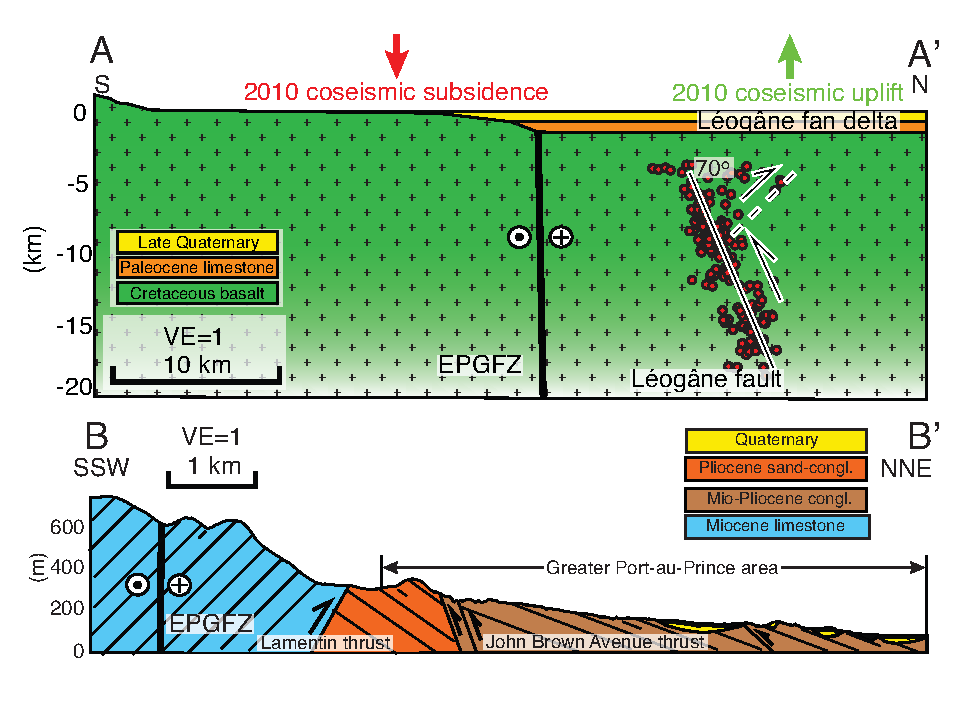
\includegraphics[width=\textwidth]{Haiti_figure3}
\caption{\textbf{Chirp sonar profiles showing the relationship of the trace of the EPGFZ and a newly described thrust we have named the Jimani thrust.} Cross sections of A, and B are indicated in Figure~\ref{figure2}A. The EPGFZ beneath Lake Azuey forms a 10 m-wide zone that can be traced as a lineament to the east and west of Lake Azuey (Figure~\ref{figure2}). The green and red horizons represent two distinguish stratigraphic layers. The two strands of the EPGFZ are buried by 0.7 m of Holocene sediment and are extrapolated to be 250 years old since their last rupture when a sedimentation rate of 2.6 mm/yr is assumed.  Folds associate with the Jimani thrust are interpreted as fault propagation folds.}
\label{figure6}
\end{figure}

\begin{figure}
\centering
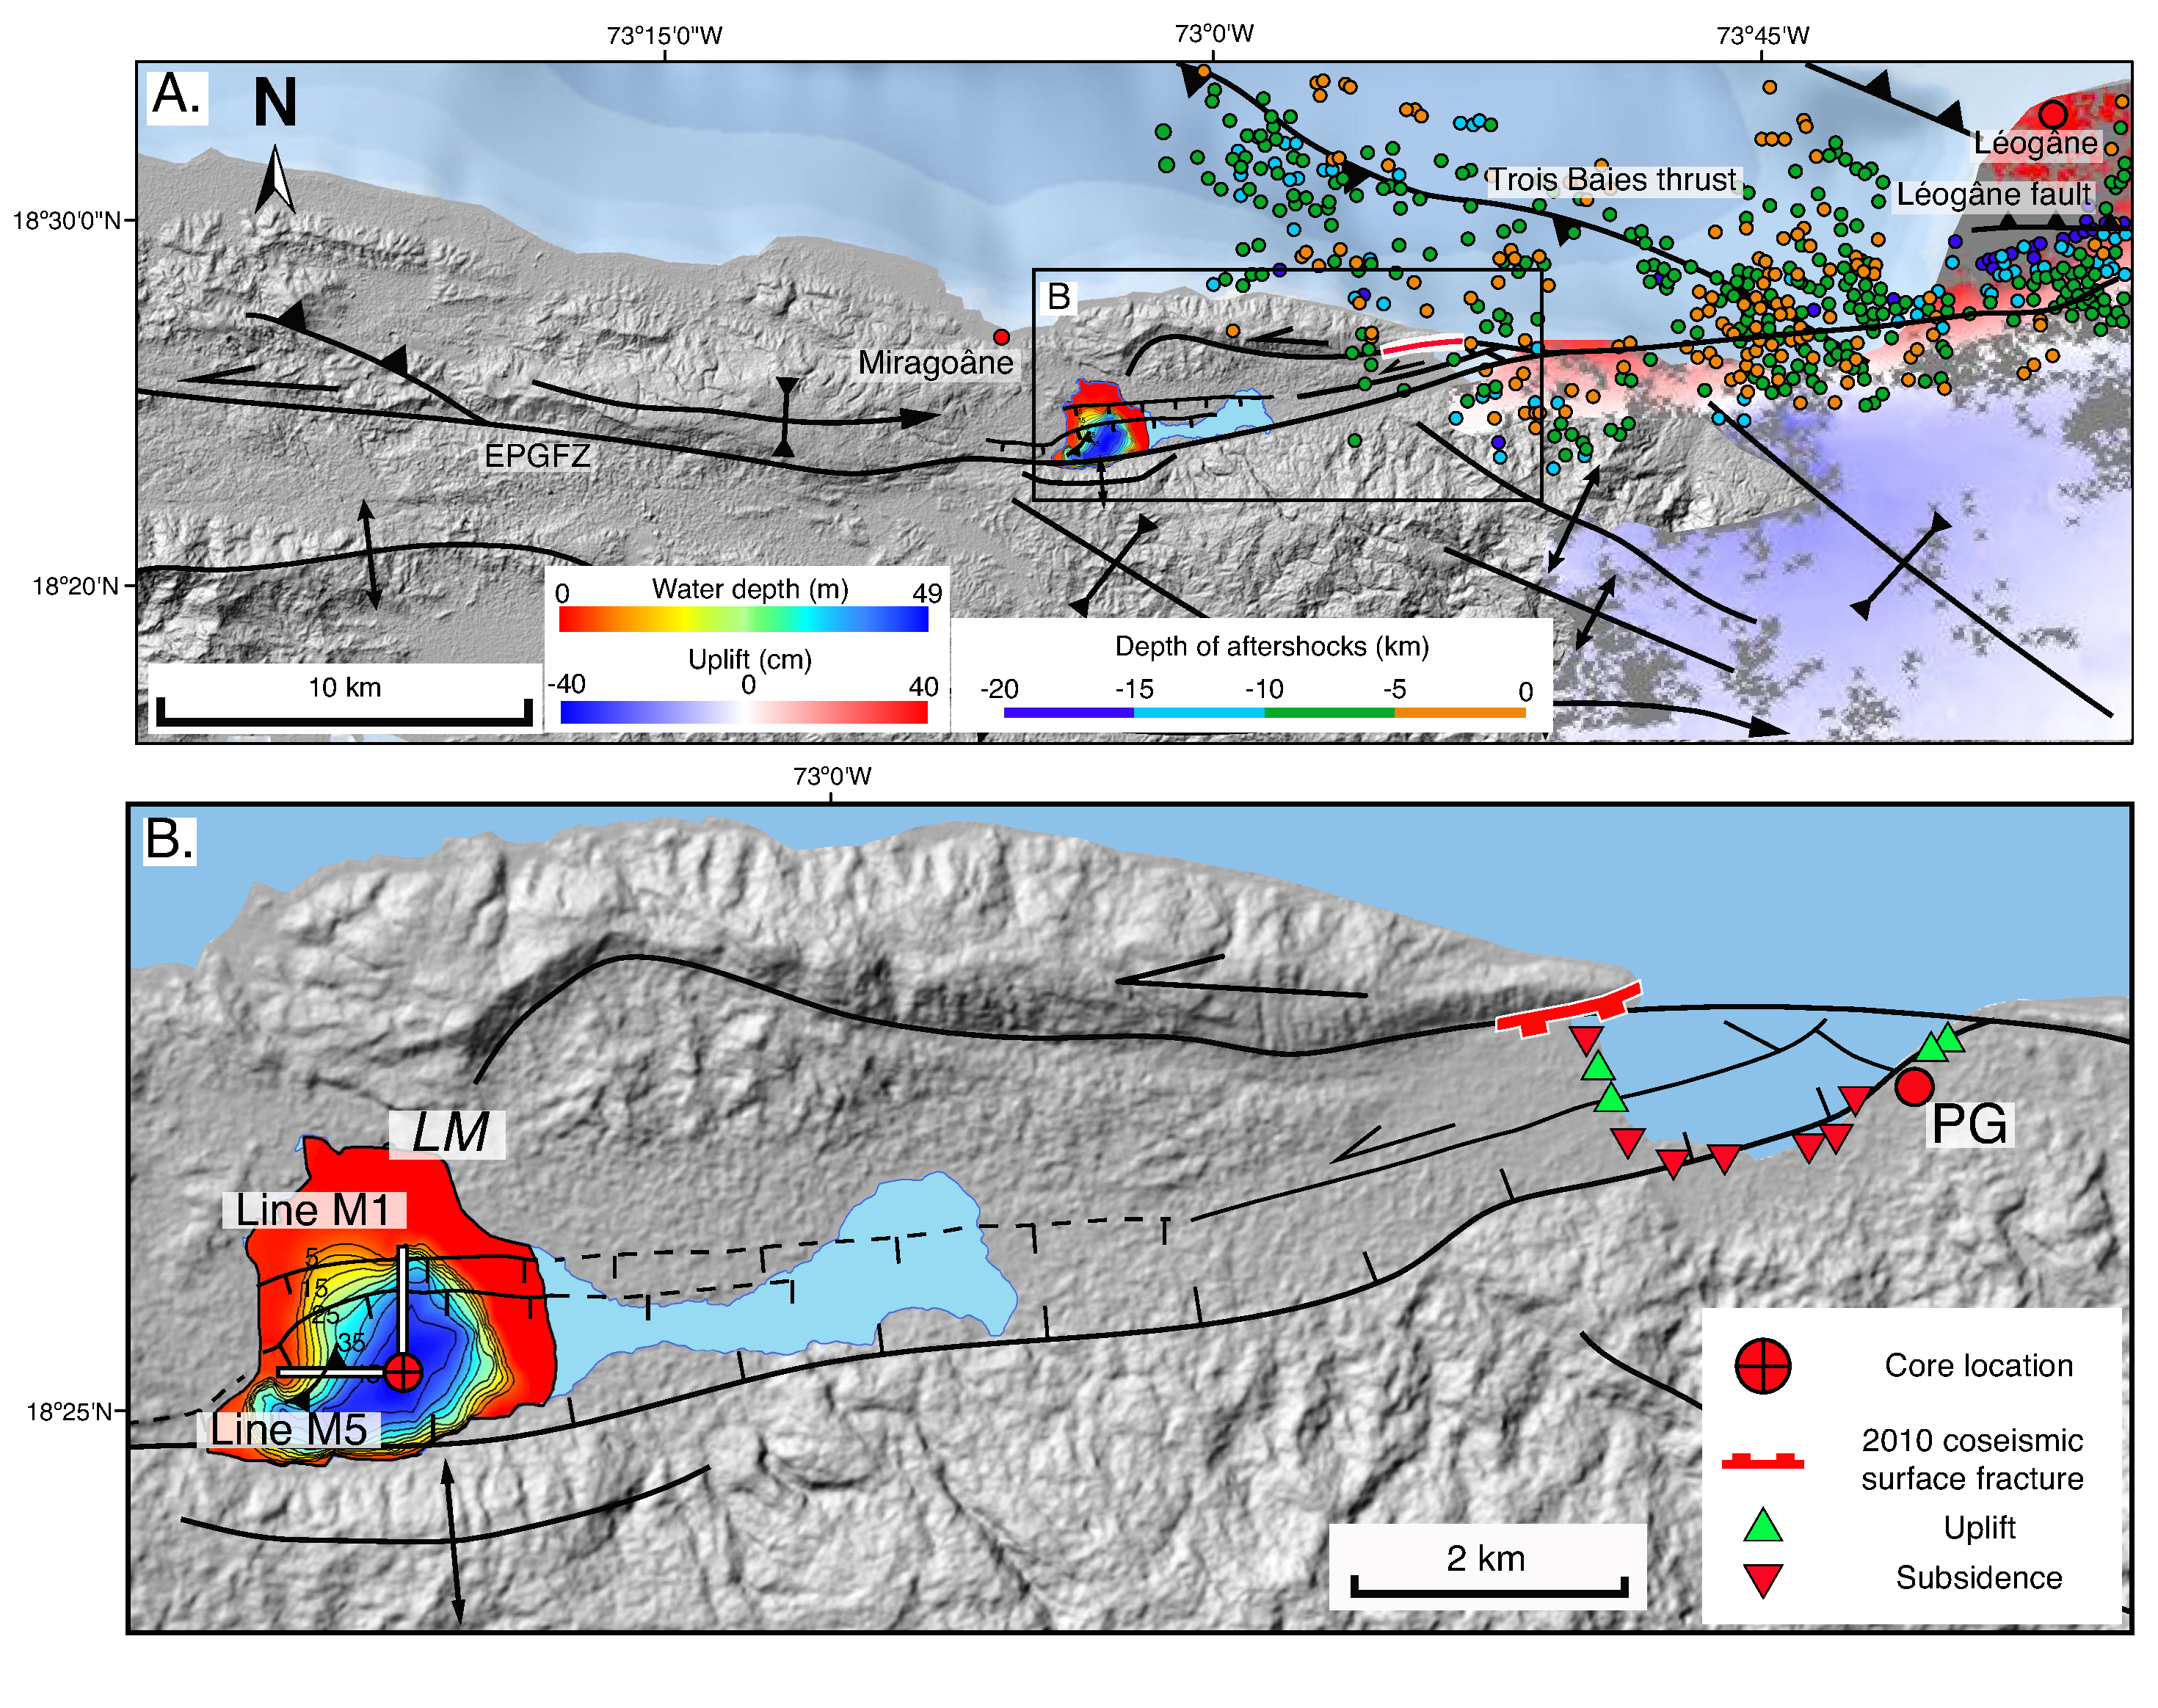
\includegraphics[width=\textwidth]{Haiti_figure7}
\caption{\textbf{Structure and 2010 coseismic surface deformation of the western segments of the EPGFZ.} \textbf{A:} Structure \citep{prentice2010seismic} and aftershock \citep{douilly2015three} map of Mirago\^ane-L\'eog\^ane region overlain with an InSAR image. \textbf{B:} Zoom of the area of Petit Goave and Lake Mirago\^ane showing the structure and bathymetry of the 14 km\textsuperscript{2}, pull-apart basin mapped beneath Lake Mirago\^ane during this study and details of the 2010 surface fracturing and coseismic subsidence in the Petit Go\^ave Bay \citep{prentice2010seismic}. \textbf{LM} = Lake Mirago\^ane; \textbf{PG} = Petit Go\^ave.}
\label{figure7}
\end{figure}

\begin{figure}
\centering
\includegraphics[width=\textwidth]{Haiti_figure8}
\caption{\textbf{Geologic setting and sonar profiles from Lake Mirago\^ane.} \textbf{A:} View looking south across the 12 km-wide and 42.8 m deep, freshwater lake. The 2 km-high, ridge along the southern edge of the lake is the scarp of the southernmost strand of the EPGFZ. The northern strand of the EPGFZ is 3 km to the north of this strand and forms the northern edge of the pull-apart basin. The core was taken by \citet{higuera199910} and was not collected from the deepest part of the lake. \textbf{B:} North-south trending line M1 (location shown on Figure~\ref{figure7}B). \textbf{C:} East-west trending line M5 (location shown on Figure~\ref{figure7}B).}
\label{figure8}
\end{figure}

\begin{figure}
\centering
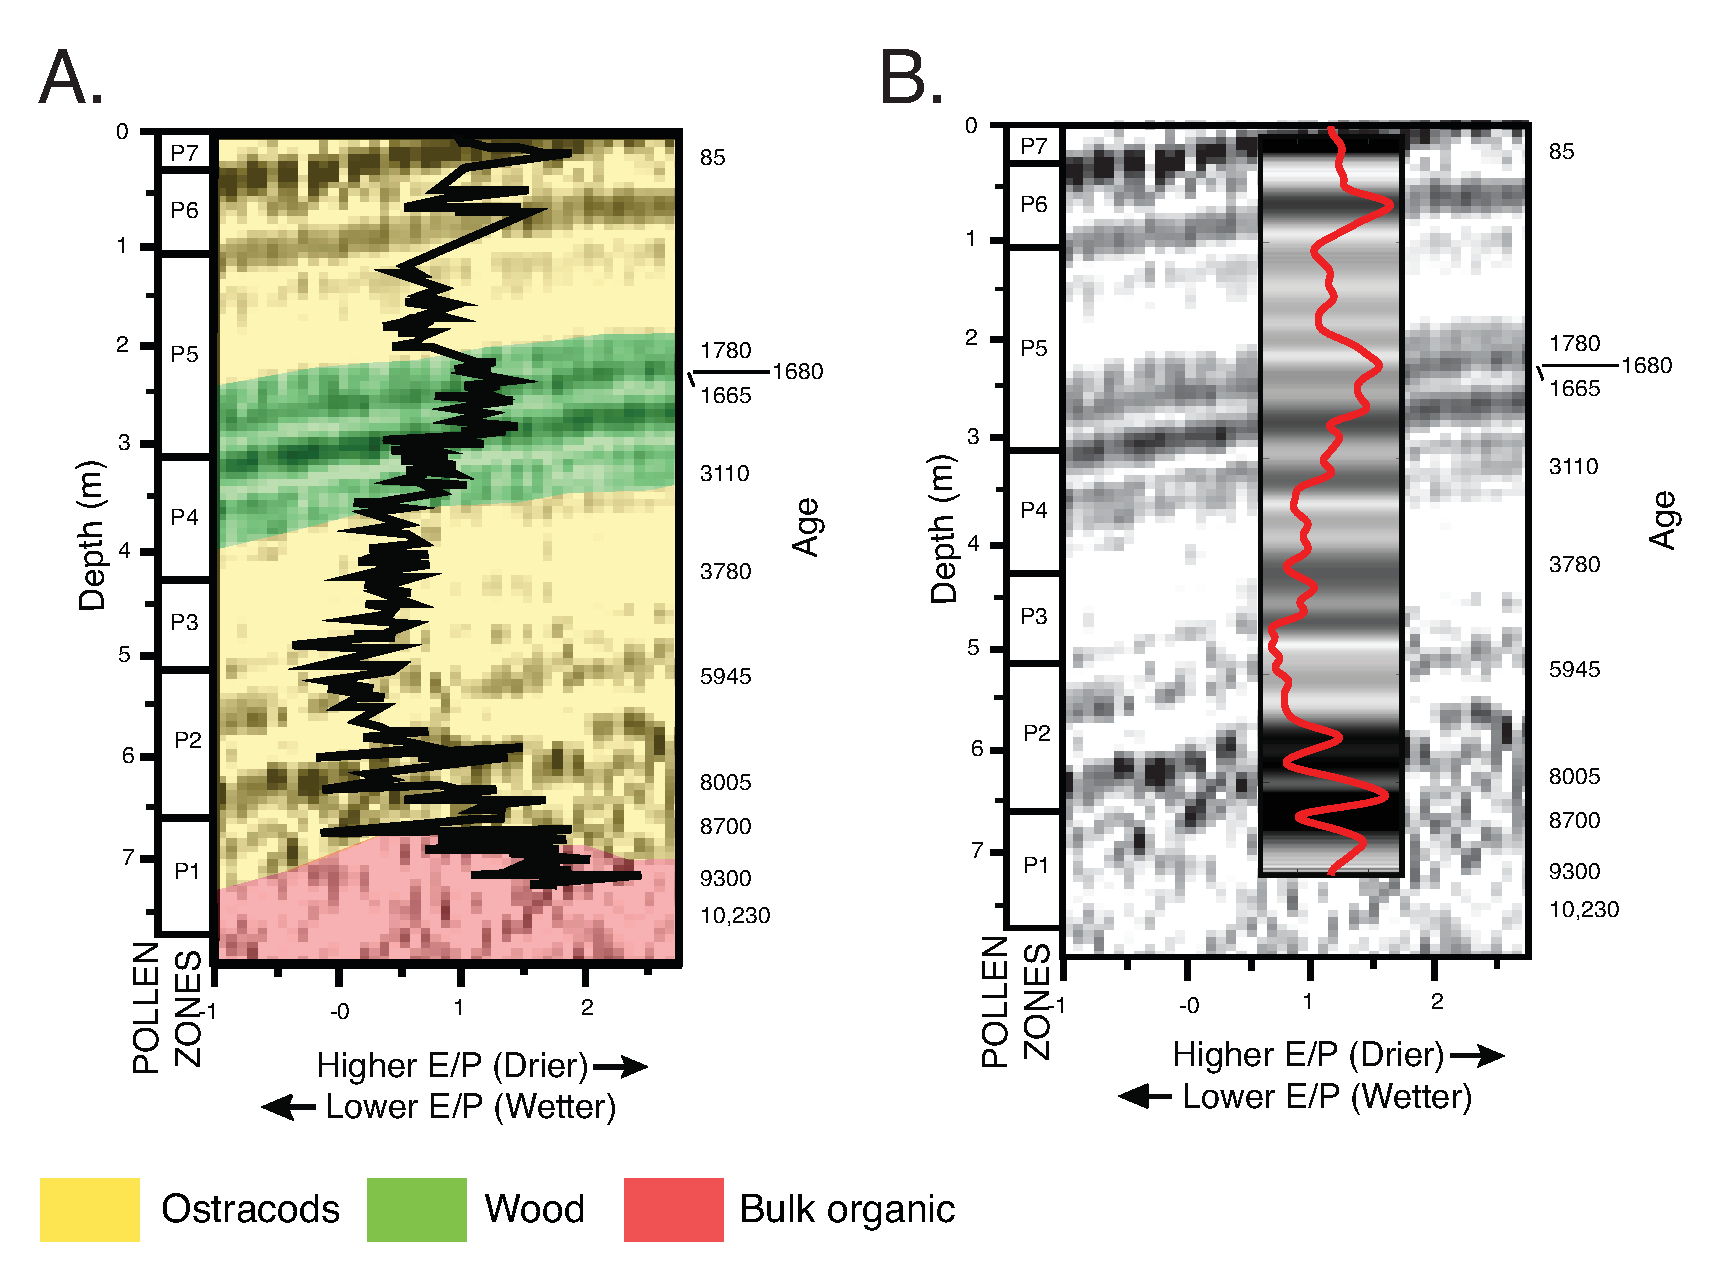
\includegraphics[width=\textwidth]{Haiti_figure9}
\caption{\textbf{Core data from Lake Mirago\^ane.} \textbf{A:} Tie between chirp sonar and core \citep{higuera199910} extending to lacustrine sediments deformed by the EPGFZ at 1770. \textbf{B:} Low-pass filtered E/P log (red) and the synthetic sonar profile generated from the low-pass filtered E/P log used as an acoustic impedance. Red bar in the Figure~\ref{figure8}A, B is the core measurement \citep{higuera199910} location.}
\label{figure9}
\end{figure}

\begin{figure}
\centering
\includegraphics[width=\textwidth]{Haiti_figure10}
\caption{\textbf{Three-dimensional block diagram showing the structural and aftershock expression of late Holocene strain partitioning in a 40-km-wide zone along a 120 km-long segment of the EPGFZ.} Black arrows show southwest direction of the Gon\^ave microplate relative to the Caribbean plate and 2010 InSAR-derived surface deformation map show and large component of shortening accommodated on a 40 km-wide zone of oblique thrusts and folds north of the EPGFZ. \textbf{PaP} = Port-au-Prince; \textbf{PG} = Petit Goave; \textbf{LA} = Lake Azuey; \textbf{LM} = Lake Mirago\^ane-L\'eog\^ane; \textbf{JF} = Jimani thrust fault; \textbf{LMF} = Lamartin thrust fault; \textbf{TBF} = Trois Baies thrust fault; \textbf{LF} = L\'eog\^ane fault. The inserted schematic diagram, modified from \citet{sibson2012reverse}. represents the conjugate thrust faults.}
\label{figure10}
\end{figure}

\begin{figure}
\centering
\includegraphics[width=\textwidth]{Haiti_figure11}
\caption{\textbf{Structural map of the San Francisco Bay region, the cos-seismic elevation and the aftershock cross-section of 1989 $M_w$ 6.9  Loma Prieta earthquake.} The cos-seismic elevation change and aftershock cross-section are modified from \citet{marshall1991faulting}}
\label{figure11}
\end{figure}

\end{document}
